\begin{figure*}
 \centering
 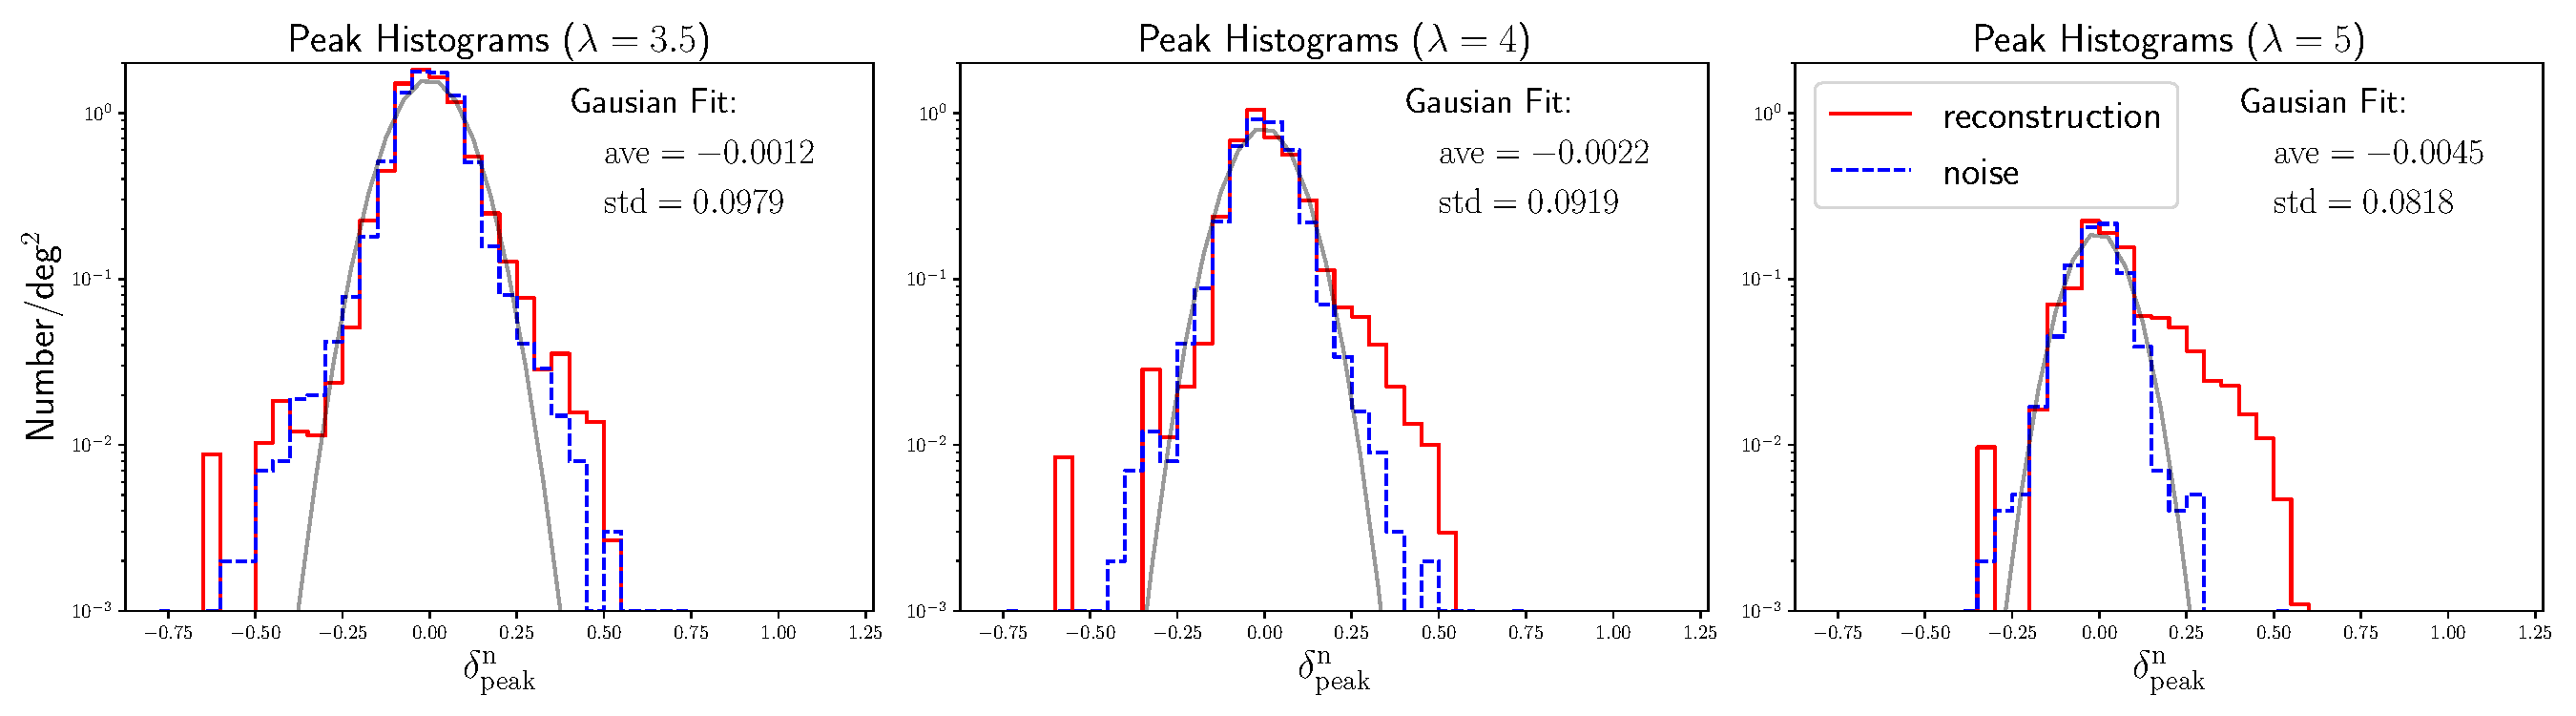
\includegraphics[width=1.0\textwidth]{peak_histograms_NFW.pdf}
 \caption{The histograms of detected peak values (normalized) from all of the
     simulations.  The solid red steps are the results from reconstructions
     with the NFW dictionary penalized with different regularization
     parameters: $\lambda=3.5,4.0,5.0$. The dashed blue steps are the
     corresponding results of the reconstructions from $1000$ realizations of
     pure noise fields. The gray lines are the best-fit Gaussian distributions
     to the noises' peak histograms.
    }\label{fig_peakHist}
\end{figure*}

In this subsection, we test the performance of our algorithm with the default
setup that models the matter density field with multi-scale NFW atoms. The
dictionary is constructed with three frames of different NFW comoving scale
radius: $0.12~h^{-1}$ Mpc, $0.24~h^{-1}$ Mpc, and $0.36~h^{-1}$ Mpc.  The
truncation radii (concentration) are set to four times the comoving scale radii
for the atoms in the dictionary. We note that each frame of our dictionary
fixes the scale radius in the comoving space; therefore, the NFW atoms have
different angular radii in different lens redshift bins.

We test the algorithm with different regularization parameters for the
preliminary lasso estimation, which are $3.5$, $4.0$, and $5.0$. The
corresponding regularization parameters for the adaptive lasso are set to
$\lambda_{\rm{als}}=\lambda_{\rm{ls}}^{\tau+1}$.  Here, we note that both the
preliminary lasso estimation and the final adaptive lasso estimation select the
pixels with the signal-to-noise ratios (SNRs) greater than $\lambda_{\rm{ls}}$
in each gradient descent iteration. While the final adaptive lasso estimation
further enhances the growth of the pixels with preliminary estimations greater
than $\lambda_{\rm{ls}}$.

This paper does not go beyond the resolution limit defined by the Gaussian
smoothing kernel with a standard deviation of $1.\arcmin 5$ and the $1\arcmin$
pixel scale as discussed in Section \ref{subsec_method_smoothing} and Section
\ref{subsec_method_pixel}, respectively.  Therefore, we smooth the
reconstructed density with the same Gaussian kernel in each lens redshift
plane.

The left panels of Figure \ref{fig_NFWvsPM} demonstrates the $3$-D density maps
reconstructed with different penalization parameters for a halo with
$M_{200}=10^{15.02} ~h^{-1}M_{\odot}$ at redshift $0.164$.  As we can see from
the reconstructed maps, the adaptive lasso algorithm sets most of the
reconstructed pixels to zero and only keeps the pixels with large amplitudes.
Therefore, it is straightforward to identify the peaks on the reconstructed
sparse density map.  Figure \ref{fig_peakHist} shows the histograms for the
detected peaks with different penalization parameters.

We simulate $1000$ realizations of pure noise fields and perform the
same reconstructions on these noise fields to study the noise properties. Figure
\ref{fig_peakHist} shows the histograms of peaks detected from the
pure noise fields. , we also find that the number of false
peaks significantly decreases as the penalization parameter increases.

\begin{figure*}
 \centering
 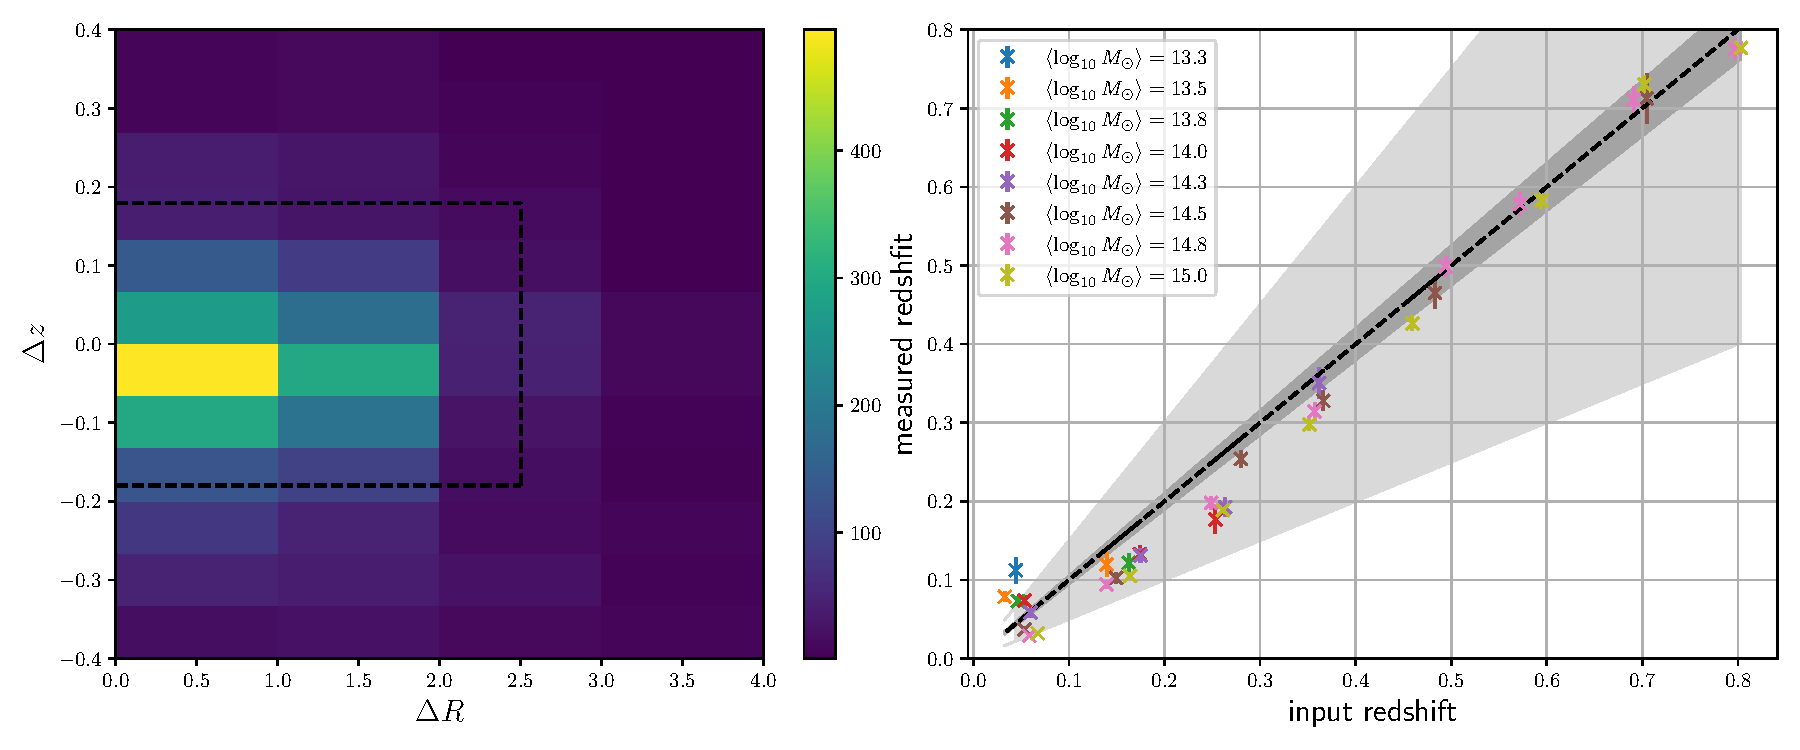
\includegraphics[width=1.0\textwidth]{peak_scatters_NFW_lbd35.pdf}
 \caption{The left panel shows the stacked $2$-D distribution of the deviations
     of detected peak positions from the centers of the corresponding input
     halos. The $x$-axis is for the deviated distance in the transverse plane,
     and the $y$-axis is for the deviation of the redshift. For each
     simulation, the positive peak inside the dashed black box with the minimal
     offset (in the pixel unit) from the input halo's position is taken as a
     true detection. The right panel focuses on the deviation of detected peaks
     in the line of sight direction. The $x$-axis is the input halo redshifts,
     and the $y$-axis is the redshift of the detected peak. The `$\cross$'
     denotes the average redshift of detected peaks for each halo over
     different noise realizations, and the error-bars are the uncertainties of
     the average redshifts. The deep gray area is for the relative redshift
     bias less than $0.05$, and the light gray area is for the relative
     redshift bias less than $0.5$. These results in this figure are based on
     the NFW dictionary with $\lambda=3.5$.
     } \label{fig_detoffsets}
\end{figure*}

The stacked $2$-D histogram, from all of the simulations, for the offsets of
the detected peak positions from the input halos' positions is shown in the
left panel of Figure \ref{fig_detoffsets}.

For each simulation, we find the positive peak closest to the input position
(in the pixel unit). If the closest peak lay inside the region denoted with
the dashed box in the left panel of Figure \ref{fig_detoffsets}, we take it as
a true peak detection of the input halo. Other detected peaks, which include both
positive and negative peaks, are taken as false peaks. The right
panel of Figure \ref{fig_detoffsets} shows the average redshift of true
detections for each halo. The estimated redshifts are lower than the true
redshifts by about $0.03$ for halos in the low-redshift range ($z\leq 0.4$).
For halos at $0.4<z\leq 0.85$, the relative redshift bias is below $0.5\%$.

\begin{figure*}
 \centering
 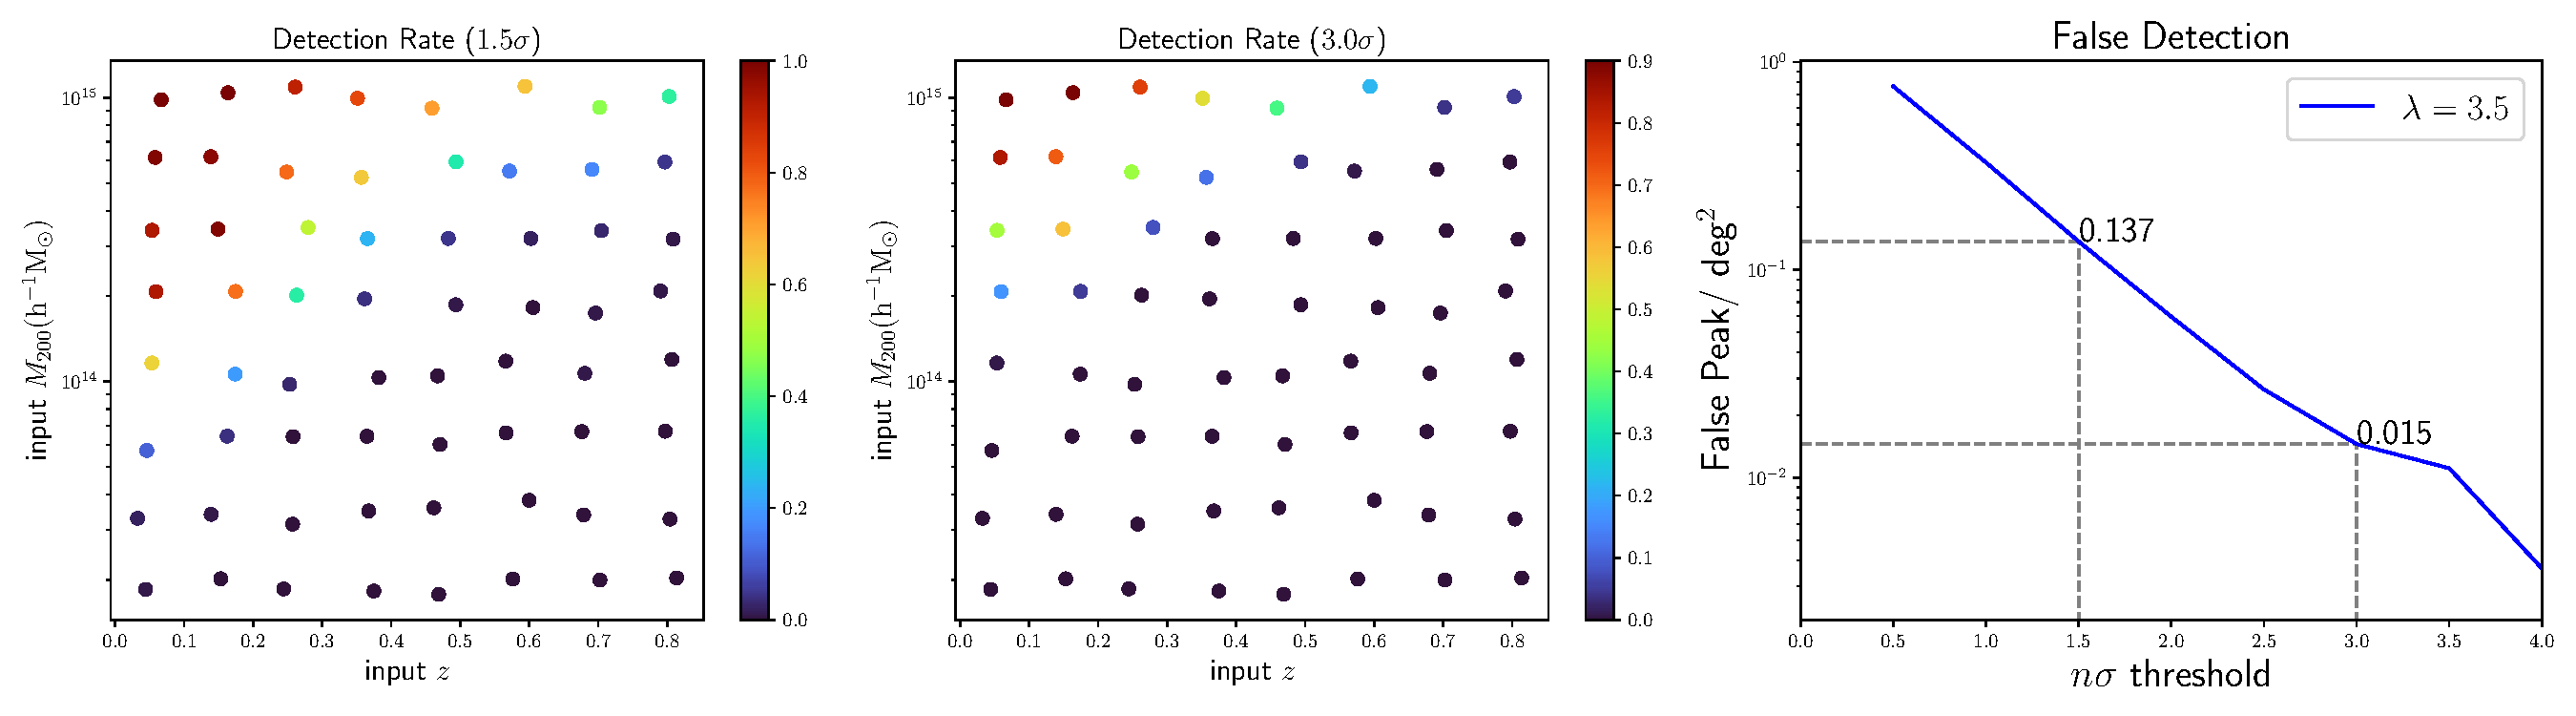
\includegraphics[width=1.0\textwidth]{detfalse_threshold_NFW_lbd35.pdf}
 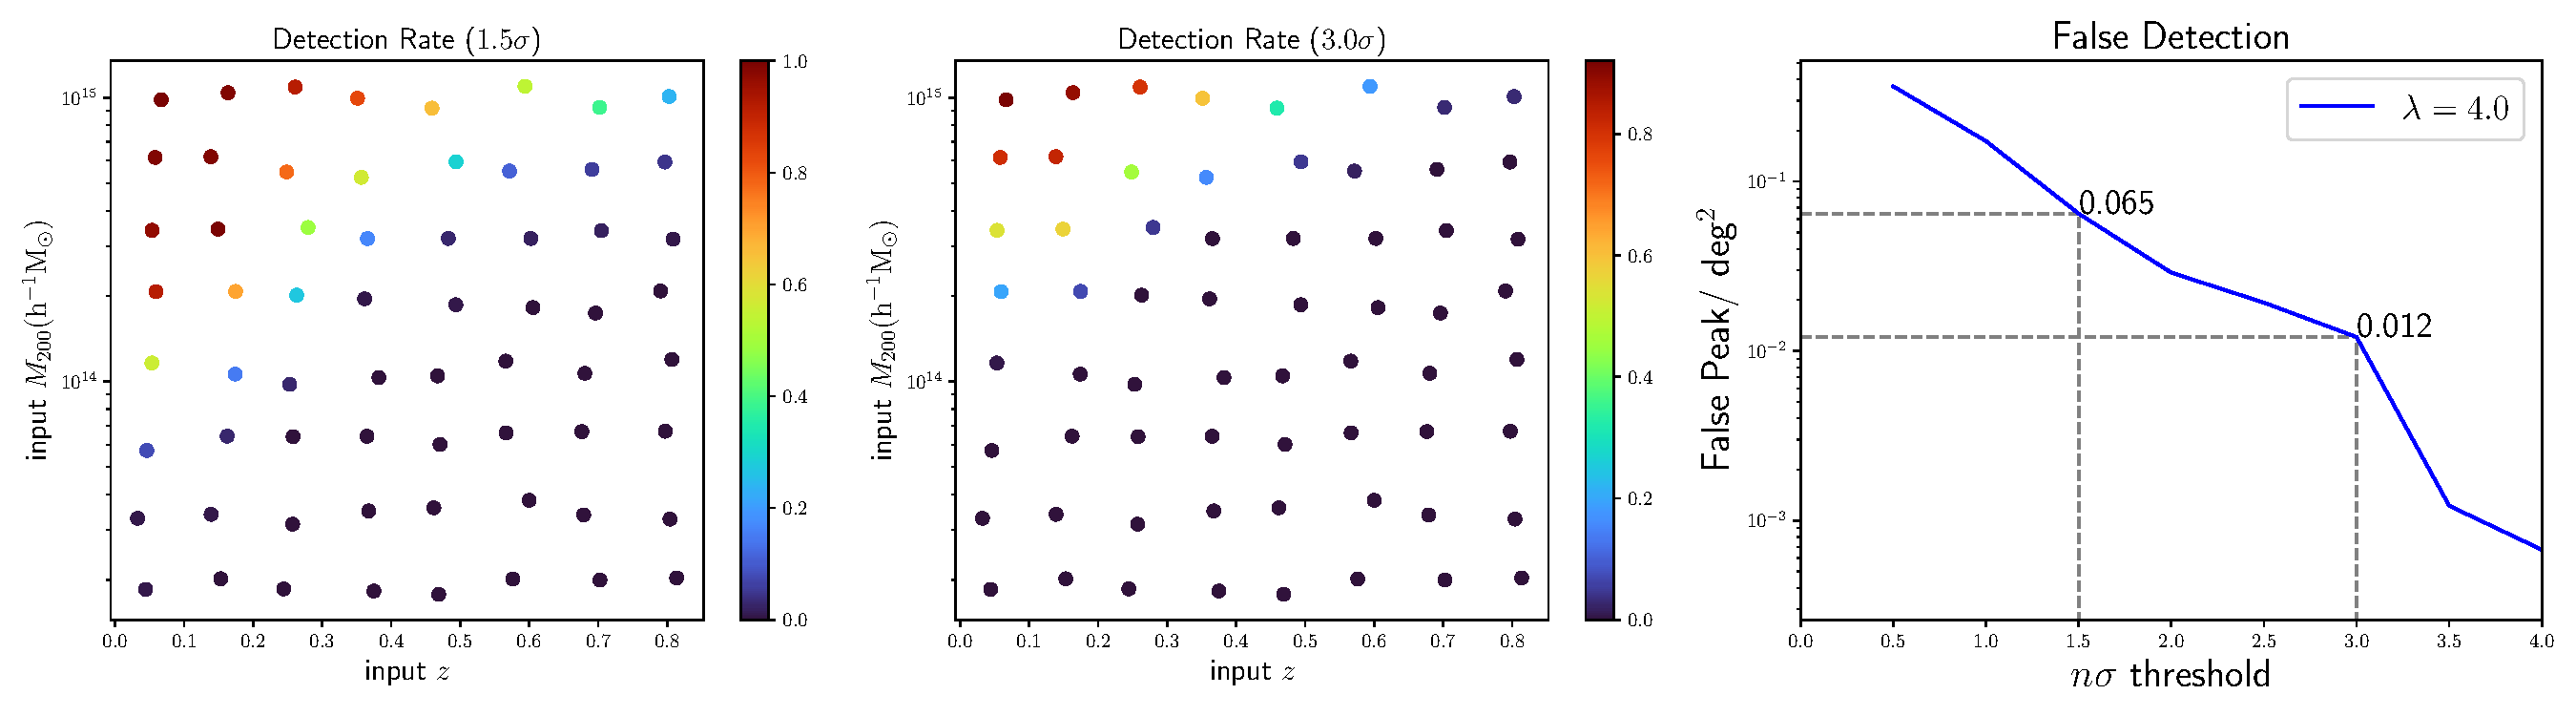
\includegraphics[width=1.0\textwidth]{detfalse_threshold_NFW_lbd40.pdf}
 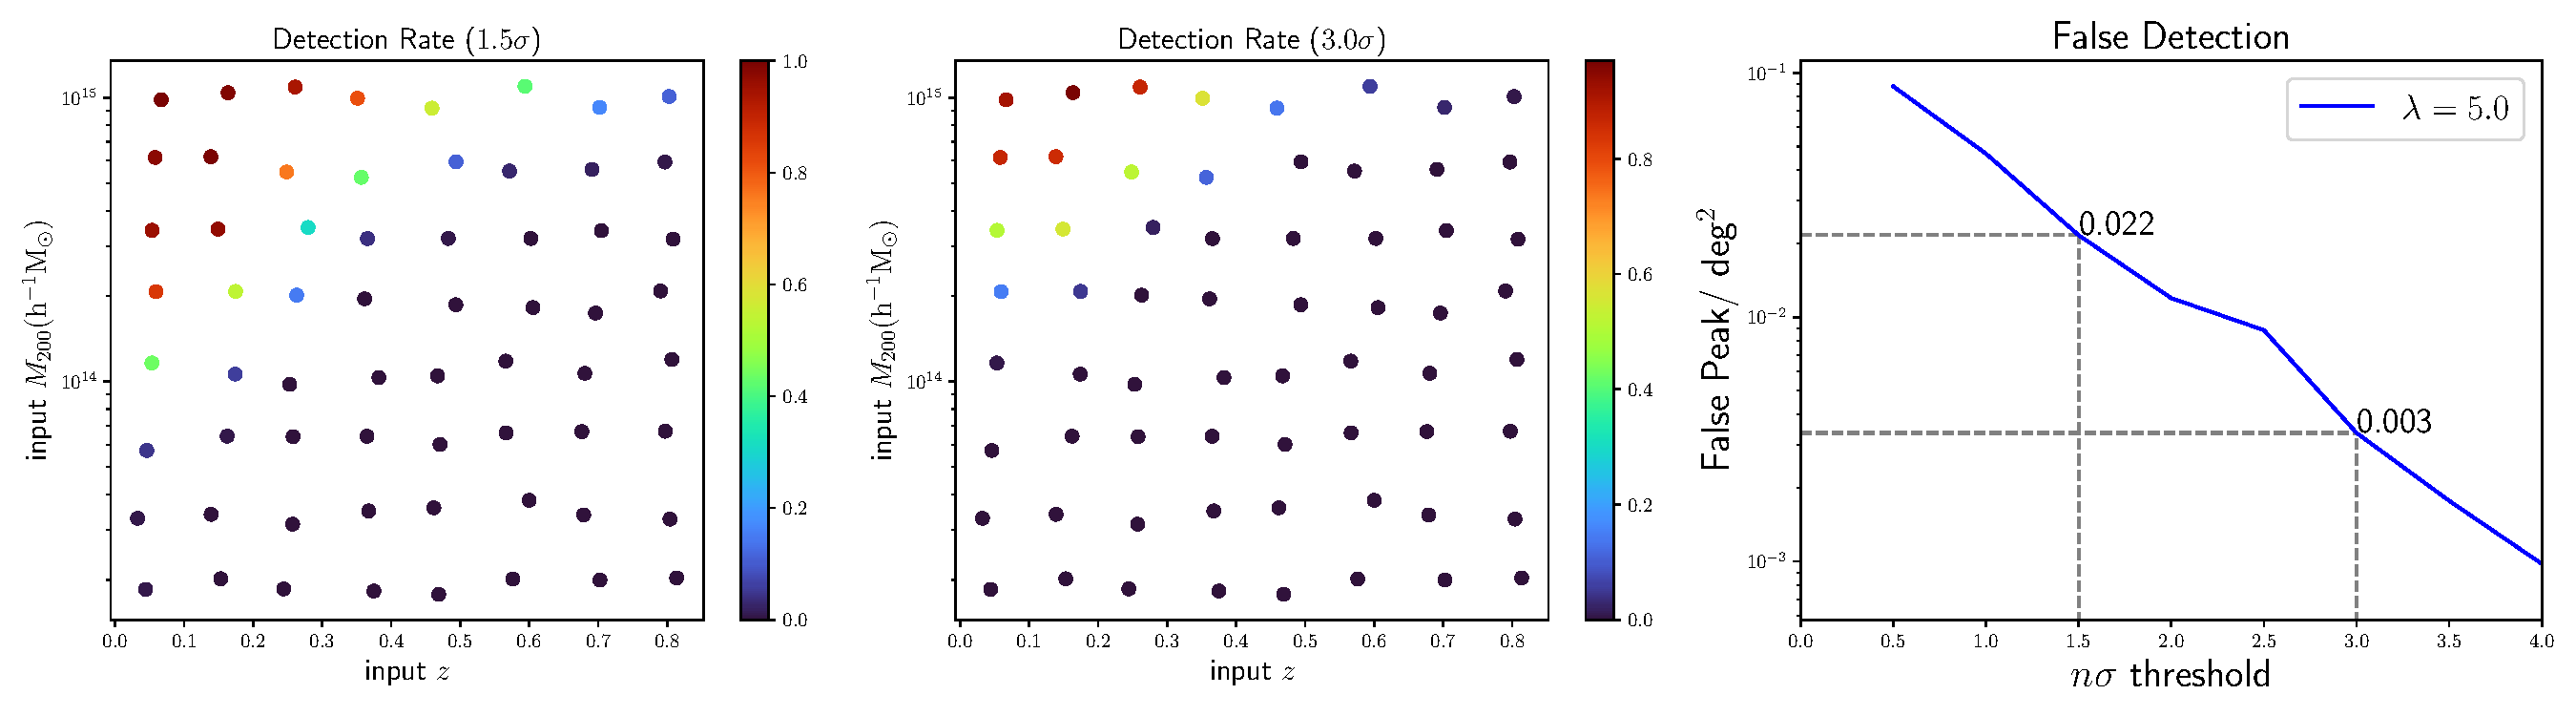
\includegraphics[width=1.0\textwidth]{detfalse_threshold_NFW_lbd50.pdf}
 \caption{The upper panels show the halo detection rate and the number of false
     peaks per square degree for mass map reconstructed with the NFW atoms. The
     penalization parameter is set to $\lambda=3.5$ for the upper panels.  The
     low panels show the results for $\lambda=5.0$.
        } \label{fig_detFalsRateNFW}
\end{figure*}

Figure \ref{fig_detFalsRateNFW} shows the detection rate (left panels) and the
number of false peaks per square degree (right panel) for each simulated halo.
The figure include results of different penalization parameters: $\lambda=3.5$
(upper panel) and $\lambda=5.0$ (lower panel).  We find that with the increase
of the penalization parameter, the detection rate decreases. On the other hand,
the number of false peaks also decreases.

